\documentclass[12pt, a4paper]{article}

\usepackage[hmargin=2.5cm, vmargin=2cm]{geometry}
\usepackage{amsthm, amssymb, mathtools, yhmath, graphicx}
\usepackage{fontspec, type1cm, titlesec, titling, fancyhdr, tabularx}
\usepackage{caption}
\usepackage{color}
\usepackage{hhline}
\usepackage{unicode-math}
\usepackage{nicefrac}

\usepackage[CheckSingle, CJKmath]{xeCJK}
\usepackage{CJKulem}
\usepackage{enumitem}
\usepackage[usenames, dvipsnames]{xcolor}
\usepackage{colortbl}
\usepackage{circuitikz}
%\setCJKmainfont[BoldFont=cwTex Q Hei]{cwTex Q Ming}
%\setCJKsansfont[BoldFont=cwTex Q Hei]{cwTex Q Ming}
%\setCJKmonofont[BoldFont=cwTex Q Hei]{cwTex Q Ming}
\setCJKmainfont[BoldFont=cwTeX Q Hei]{cwTeX Q Ming}

\def\normalsize{\fontsize{12}{18}\selectfont}
\def\large{\fontsize{14}{21}\selectfont}
\def\Large{\fontsize{16}{24}\selectfont}
\def\LARGE{\fontsize{18}{27}\selectfont}
\def\Huge{\fontsize{20}{30}\selectfont}

\titleformat{\section}{\bf\Large}{\arabic{section}}{24pt}{}
\titleformat{\subsection}{\large}{\arabic{subsection}.}{12pt}{}
\titlespacing*{\subsection}{0pt}{0pt}{1.5ex}

\parindent=24pt

\DeclarePairedDelimiter{\abs}{\lvert}{\rvert}
\DeclarePairedDelimiter{\norm}{\lVert}{\rVert}
\DeclarePairedDelimiter{\inpd}{\langle}{\rangle}
\DeclarePairedDelimiter{\ceil}{\lceil}{\rceil}
\DeclarePairedDelimiter{\floor}{\lfloor}{\rfloor}

\newcommand{\unit}[1]{\:(\text{#1})}

\title{ \bf {\huge 電子電路實驗三:類比電表之內電阻及擴大測量範圍之方法}\\ 實驗預報}
\author{B02901178 江誠敏}
\date{2014/09/21}

\begin{document}

\maketitle

\section{預報問題}

\begin{enumerate}[itemsep=20pt, topsep=10pt]
	\item {\large 圖3.7(a)中,伏特計內電阻$R_0$,請推導伏特計讀值$V_0$與電源供應器供應電位差$E$之關係。} \\[10pt]

		\begin{center}
			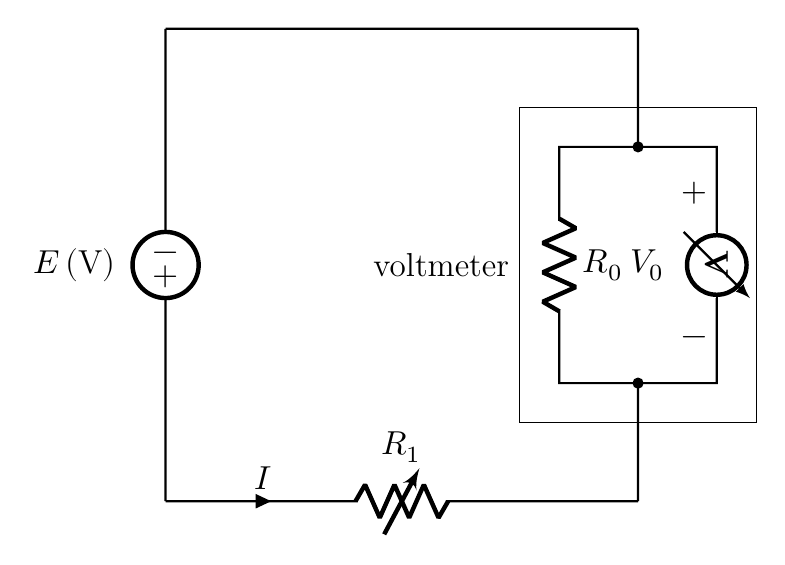
\begin{tikzpicture}[american voltages, scale=1]
				\draw[color=black, thick]
				(0, 0) to [V=$E \unit{V}$] (0, 6) 
				(0, 0) to [vR, l=$R_1$, i>^=$I$] (6, 0) 
				(6, 0) to [short, -*] (6, 1.5)
				(6, 1.5) -| (5, 1.5) to [R, l_=$R_0$] (5, 4.5) |- (6, 4.5) 
				(6, 4.5) -| (7, 4.5) to [voltmeter, v_=$V_0$] (7, 1.5) |- (6, 1.5)
				(6, 4.5) to [short, *-] (6, 6)
				(6, 6) to [short] (0, 6)
				;
				\draw (4.5, 1) rectangle (7.5, 5);
				\draw (3.5, 3) node{voltmeter};
			\end{tikzpicture}
		\end{center}

		對整個電路,由KVL可以得到$E - IR_1 - IR_2 = 0$,因此有$I = \dfrac{E}{R_1 + R_0}$,而$V_0$等於電阻$R_1$的跨壓,$V_0 = I R_0 = \dfrac{R_0}{R_0 + R_1} E$。

	\item {\large 圖3.7(b)中,安培計內電阻$R_0$,請推導安培計讀值$I_0$與電源供應器供應電流$I$之關係。} \\[10pt]

		\begin{center}
			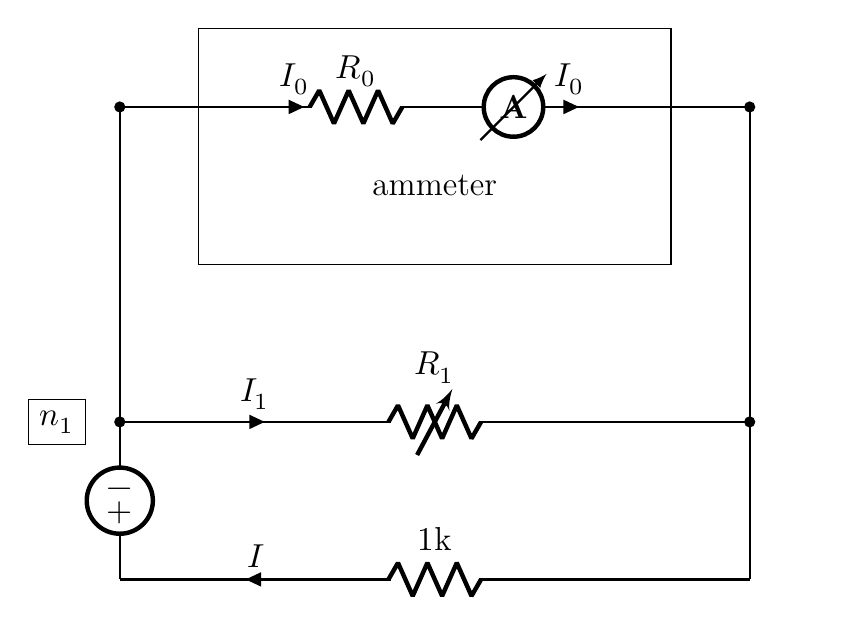
\begin{tikzpicture}[american voltages, scale=1]
				\draw[color=black, thick]
				(0, 0) to [V] (0, 2) 
				(0, 2) to[short] (0, 6)
				(0, 6) to[short, *-] (2, 6)
				(2, 6) to[R, l=$R_0$, i>^=$I_0$] (4, 6)
				(4, 6) to[ammeter, i=$I_0$] (6, 6)
				(6, 6) to[short, -*] (8, 6)
				(0, 2) to[vR, l=$R_1$, i>^=$I_1$, *-*] (8, 2)
				(8, 6) to[short] (8, 0)
				(0, 0) to[R, l=$1$k, i<^=$I$] (8, 0)
				;
				\draw (1, 4) rectangle (7, 7);
				\draw (4, 5) node{ammeter};
				\draw (-0.8, 2) node[rectangle, draw, text centered]{$n_1$};
				\draw (9, 2) node{};
			\end{tikzpicture}
		\end{center}

			對節點$n_1$用KCL可以得到$I = I_0 + I_1$,但由最上面的mesh loop,$I_0 R_0 = I_1 R_1$,所以$I = I_0 + I_0 \dfrac{R_0}{R_1}$,因此$I_0 = \dfrac{R_1}{R_0 + R_1} I$

	\end{enumerate}

	\end{document}

